\chapter{(Network) Flow Problems}

\begin{descr}
    TODO
\end{descr}

\section{Network Flow Problems}\index{Network Flow Problems}
\begin{example}
Example: Oil field + transportation

\end{example}

\begin{definition}
A network N consists of 
\begin{enumerate}
\item A finite directed graph $G=(V,E)$ without loops and parallel edges
\item a function $c: E -> \mathds{R}^{+}$, which assigns a capacity to each edge
\item two designated nodes s and t, called \deftxt{source} and \deftxt{sink}
\end{enumerate}
Short: $N = (G, c, \{s, t\})$
\end{definition}

\begin{definition}
Let $N = (G, c, \{s, t\})$ be a network. A flow function on N is a function $f: E -> \mathds{R}$ such that 
\begin{itemize}
\item $ 0 \le f(e) \le c(e), \forall e \in E $
\item $ \alpha(v) := \{e:$ endpoint of e is v $\}, v \in V$ \\
$\beta(v) := \{e:$ startpoint of e is v $\}, v \in V$
\end{itemize}
For every $v \in V\backslash\{s, t\} $ \\
$ \sum_{e \in \alpha(v)} f(e) = \sum_{e \in \beta(v)} f(e) $ \\
This is called \deftxt{"conservation function"}. \\
The \deftxt{total flow} of the flow function is given by $F = \sum_{e \in \alpha(t)} f(e) - \sum_{e \in \beta(t)} f(e) $
\end{definition}

\begin{example}
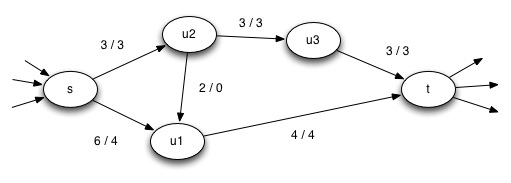
\includegraphics{diagrams/Chapter3_Example1.jpg}
\\Notion: $ 6 / 4 $ describes the capacity and the flow of an edge. In this example the capacity of the edge is 6 and the flow is 4.
\end{example}

Problem: \\
Given an arbitrary network N, find a flow function f, where the total flow F is maximal. \\

\begin{definition}
Let N = $(G, c, \{s, t\})$ be a network. Let $S \subseteq V$ with s $\in S, t \notin S$ \\
$\bar{S} = V \backslash S$ (i.e. $t \in \bar{S}$) \\
$E_{S\bar{S}} = \{e:$ all edges with starting point in S and endpoint in $\bar{S} \}$ \\
$E_{\bar{S}S} = \{e:$ all edges with start point in $\bar{S}$ and end point in S $\}$ \\
$E_{S\bar{S}} \cup E_{\bar{S}S} $ is the \deftxt{cut} defined by S. \\
The capacity of a cut defined by S: $c(S) = \sum_{e \in E_{\bar{S}S}}c(e)$
\end{definition}

\begin{lemma}
Let $N =(G, c, \{s, t\})$ be a network, $f: E \rightarrow \mathds{R}$ be a flow function then for any $S \subseteq V$ with $s \in S, t \notin S$: 
\[
F = \sum_{e \in E_{S\bar{S}}}f(e) - \sum_{e \in E_{\bar{S}S}} f(e)
\]
\end{lemma}

\begin{proof}
\[ F = \sum_{e \in \alpha(t)} f(e) - \sum_{e_ \in \beta(t)} f(e) \]
\[0 = \sum_{e \in \alpha(v)} f(e) - \sum_{e \in \beta(v)} f(e); \forall v \in \bar{S} \backslash \{t\} \]
We add all these equations up. Left hand side: $F$ remains. Right hand side: Let $x \xrightarrow{e} y$ be an edge. We need to consider 4 cases:
\begin{enumerate}
\item $x, y \in S$, then the value $f(e)$ does not occur in the summation
\item $x, y \in \bar{S}$, then $f(e)$ occurs one time positive in the summation, namely for y \\ f(e) occurs one time negative in the summation, namely for x 
\item $x \in S; y \in \bar{S}$, f(e) occurs positive for y and nowhere else and $e \in E_{S\bar{S}}$
\item $x \in \bar{S}; y \in S$, then $f(e)$ occurs negative for x and nowhere else and $e \in E_{\bar{S}S}$
\end{enumerate}
This leads to the following equation:
\[F = \sum_{e \in E_{S\bar{S}}}f(e) - \sum_{e \in E_{\bar{S}S}} f(e) \]
Only case 3 are 4 contribute.
\end{proof}

\begin{lemma}
For every flow function f with total flow F and any ser $S \subseteq V$, $s \in S$, $t \notin S$
$$ F \le c(S) $$
\end{lemma}

\begin{proof}
From lemma 3.1 we know
\[F = \sum_{e \in E_{S\bar{S}}}f(e) - \sum_{e \in E_{\bar{S}S}}f(e) \le \sum_{e \in E_{S\bar{S}}}f(e) \le \sum_{e \in E_{S\bar{S}}}c(e) = c(S) \] 
\end{proof}

\begin{corollary}[Max Flow - Min Cut Statement]
If $F=c(S)$ then the total flow F is \underline{maximal} and the capacity of the cut defined by $S$ is \underline{minimal}.
\end{corollary}

\begin{proof}
Let $F = c(S)$, consider another flow function $f'$ with total flow $F'$.
\begin{enumerate}
\item $F' \le c(S)$ (Lemma 3.2) // $F' \le c(S) = F$ \\Hence, f is a flow function with maximal total flow.
\item Let $S'$ with $s \in S'$, $t \notin S'$ be given. $c(S) = F \le c(S')$. Hence the capacity $c(S)$ is minimal among all other capacities. 
\end{enumerate}
\end{proof}

An \deftxt{augmenting path} is a simple path from s to t, that is not necessarily directed. And for which the following two cases hold: Let e be an edge on this path: 
\begin{enumerate}
\item $ s \rightarrow \circ \rightarrow \circ \rightarrow ... \rightarrow \underset{s_i}{\circ} \xrightarrow{e} \underset{s_{i+1}}{\circ} ...  \underset{t}{\circ}$ then we request that $f(e) < c(e)$
\item $s \rightarrow \circ ...  \underset{s_i}{\circ} \xleftarrow{e} \underset{s_{i+1}}{\circ} ... \underset{t}{\circ}$ then we request that $f(e) > 0$
\end{enumerate}

\begin{example}
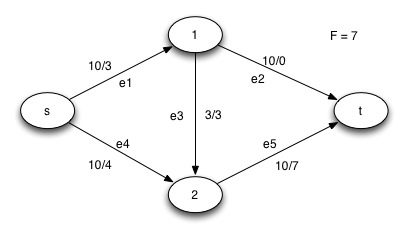
\includegraphics{diagrams/Chapter3_Example2.jpg} \\
Which of the following is an augmenting path? 
\begin{itemize}
\item $e_1 e_2$
\item $e_1 e_3 e_5$
\item $e_4 e_3 e_2$
\item $e_4 e_5$
\end{itemize}

Solution: \\
The first, third and fourth example are augmenting paths. The second path violates case 1.
\end{example}

We use $e_4 e_3 e_2$ to improve the flow function as follows:
\begin{itemize}
\item For forward egdes $e: c(e) - f(e)$:
\begin{itemize}
	\item $e_4: 6$
	\item $e_2: 10$
\end{itemize}
\item For backward edges $e: f(e)$
\begin{itemize}
\item $e_3: 3$
\end{itemize}
\end{itemize}
We chose the minimum from the values and add the value to the flow of forward egdes and substract it from backward egdes. The flows of the edges change as follows:
\begin{itemize}
\item $e_4 = \xfrac{10}{7}$
\item $e_2 = \xfrac{10}{3}$
\item $e_3 = \xfrac{3}{0}$
\end{itemize} 

\begin{example}
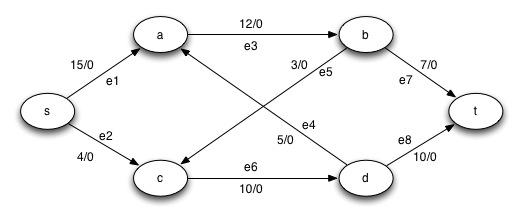
\includegraphics{diagrams/Chapter3_Example3.jpg} \\
Augmenting path: \\
$s* \xrightarrow{e_2} c* \xrightarrow{e_6} d* \xrightarrow{e_4} a* \xrightarrow{e_3} b* \xrightarrow{e_7} t*$ \\
Compute deltas:
\begin{itemize}
\item $\Delta_{(e_2)} = 4$
\item $\Delta_{(e_6)} = 10$
\item $\Delta_{(e_4)} = 5$
\item $\Delta_{(e_3)} = 12$
\item $\Delta_{(e_7)} = 7$
\end{itemize}
The minimum $\Delta$ is 4, so the flow of the edges will be increased by 4.
\begin{itemize}
\item $e_2 = \xfrac{4}{4}$
\item $e_6 = \xfrac{10}{4}$
\item $e_4 = \xfrac{5}{4}$
\item $e_3 = \xfrac{12}{4}$
\item $e_7 = \xfrac{7}{4}$
\end{itemize} 

The next steps or paths would be:
\begin{itemize}
\item $s \rightarrow a \rightarrow b \rightarrow c \rightarrow d \rightarrow t$
\item $s \rightarrow a \rightarrow b \rightarrow t$
\item $s \rightarrow a \rightarrow d \rightarrow t$
\end{itemize}
The application of this paths leads to a new flow: $F = 14$.
\end{example}

\begin{lemma}
When executing a step in the algorithm, the actual function f is a flow function.
\end{lemma}

\begin{proof}
The assumption is obviously true for step 1 because $f \equiv 0$ is a flow function. It is obviously true for steps 2, 3 and 5, too, because f is not modified. \\
Step 4: \\
Let $f$ be a flow function when we enter step 4. We have to show that after performing step 4, the newly calculated function $f$ is still a flow function. \\
Let $f_{old}$ be the function with which we enter step 4 and $f_{new}$ the newly calculated one. $f_{old}$ is a flow function. Hence, 
\[\sum_{e \in \alpha(v)} f_{old}(e) = \sum_{e \in \beta(v)}f_{old}(e); \forall v : v \neq s, v \neq t\]
Let $s \rightarrow v_0 \rightarrow v_1 ... v_{f_{e-1}} \rightarrow v_{f_e} \rightarrow t$ be an augmenting path used in step 4. By definition of $\Delta f_{new}(e) < c(e)$ and $f_{new}(e) > 0$. \\
For step 4: Let $s = v_0 \rightarrow ... \rightarrow v_2 = t$ be the path along which we achieved the marking. Only the flow value of the edges along this path is modified, so we have to check only the edges respectively nodes along this path. We have to check: 
\begin{enumerate}
\item $ 0 \le f_{new}(e) \le c(e) \forall e$: e edge on the path
\item $\sum_{e \in \alpha(v)} f_{new}(e) = \sum_{e \in \beta(v)}f_{new}(e),  \forall v$, v on the path, $v \neq s, v \neg t$ 
\end{enumerate}
The check: 
\begin{enumerate}
\item 1 holds by the definition of $\Delta$
\item Let $v_i, v_i \neq s, v_i \neq t$ be a node on the path:
\begin{enumerate}
\item $\xrightarrow{e_i} v_i \xrightarrow{e_{i+1}}, e_i \in \alpha(v_i), e_{i+1} \in \beta(v_i)$ for both edges $f_{new}$ is obtained from $f_{old}$ by adding $\Delta$, so 2 holds in this case
\item $\xrightarrow{e_i} v_i \xleftarrow{e_{i+1}}, e_i, e_{i+1} \in \alpha(v_i)$. One contributes $\Delta$, the other contributes $-\Delta$, so 2 holds for $v_i$
\item $\leftarrow v_i \leftarrow$ analogously
\item $\leftarrow v_i \rightarrow$ analogously, too
\end{enumerate}
\end{enumerate}
\end{proof}

\begin{lemma}
If the algorithm by Ford-Fulkerson terminates then the determined flow function has maximal total flow.
\end{lemma}

\begin{proof}
If the algorithm terminates, then it does so in step 3. That means we started labeling but did not reach $t$. Let $S$ be the set of nodes that were marked in the last round. Then $s \in S$ and $t \notin S$. $\bar{S} = V \backslash S$. Let $x \xrightarrow{e} y$ be an edge in $E_{S\bar{S}}$, this means x is labelled, y is not labelled. So, we know that $f(e) = c(e)$ because otherwise we could have marked y.\\
If $x \xrightarrow{e} y$ is an edge in $E_{\bar{S}S}$ ($x \in \bar{S}, y \in S$). So, $y$ is labelled and $x$ is not. Then we can conclude that $f(e) = 0$, otherwise we could have marked $e$. 
\[F \stackrel{(3.1)}{=} \sum_{e \in E_{S\bar{S}}}f(e) - \underbrace{ \sum_{e \in E_{\bar{S}S}}f(e)}_{= 0} = \sum_{e \in E_{S\bar{S}}} c(e) = c(e) \]
f is a flow function with maximal total flow. 
\end{proof}

\deftxt{Termination} \\

\begin{lemma}
If $c: E -> \N$ then the algorithm terminates.
\end{lemma}

\begin{proof}
This holds because the algorithm starts with $f \equiv 0$ and the total flow $F$ is increased by $\Delta$ and $\Delta$ is a natural number as $c(e) \in \N \forall e$ and because $F \le c(s)$ for all $S$ with $s \in S, t \notin S$ i.e. F is bordered. \\
What about $c: E -> \R$? 
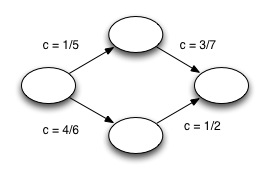
\includegraphics{diagrams/Chapter3_Proof_3_6.jpg} \\
Turn the capacities into natural numbers, calculate the results and divide them later.
\end{proof}

\begin{proposition}
The example with $c: E -> \R \backslash \Q$ is an example, for which we can apply the algorithm in a way that is does not terminate. 
\end{proposition}

\begin{example}
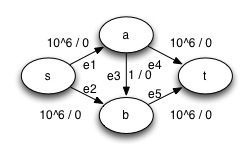
\includegraphics{diagrams/Chapter3_Example_4.jpg} \\
Maximal total flow: $2 * 10^6$ \\
Selecting the augmenthing paths: 
\begin{itemize}
\item $e_1 e_4$ 
\item $e_2 e_5$
\end{itemize}
This would solve the problem within two steps, but... \\
Choosing the following augmenting paths: 
\begin{itemize}
\item $e_1 e_3 e_5$ with $\Delta = 1$ and
\item $e_2 e_3 e_4$ with $\Delta = 1$ 
\end{itemize}
would lead to $2*10^6$ rounds to solve the problem. 
\end{example}

\begin{theorem}
If we use breadth-first-search when labelling and always select the shortest augmenting pathe, then the algorithm terminates and uses $O(|V|^3 * |E|)$ steps for any $c:E -> \R$ (where it is assumed that any real number can be manipulated in one step).
\end{theorem}

\begin{definition}
Let e be an edge between u and v with flow value $f(e)$. e is called \deftxt{useful} from u to v if 
\begin{enumerate}
\item $ u \xrightarrow{e} v$ and $f(e) < c(e)$
\item $u \leftarrow v$ and $f(e) > 0 $
\end{enumerate}
Let $G = (V,E)$ be the directed graph for the network and $f$ a flow function for the network. A \deftxt{layering} for the network is defined as follows: 
\begin{enumerate}
\item $V_0 = \{s\}, i \leftarrow 0$
\item $ T := \{ v \in V, v \notin V_j, j \le i$ and there is an useful edge from a node in V to v $\}$
\item If $ T = \emptyset$ then the actual flow function has maximal total flow and the algorithm stops. 
\item If $t \in T$ then put $l := i+1, V_l = \{t\}$ and stop the algorithm.
\item $V_{i+1} := T, i \leftarrow i+1$ and go to step 2
\end{enumerate}
$E(i) = \{e$: e is an useful edge between some node in $V_{n-1}$ and $V_i \}$
\end{definition}

\begin{example}
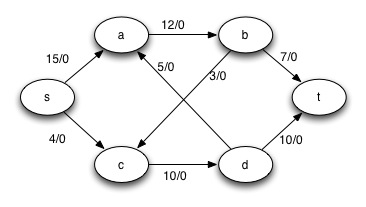
\includegraphics{diagrams/Chapter3_Example5.jpg} \\
Layers:
\begin{itemize}
\item $V_0 = \{s\}$
\item $V_1 = \{a, c \}$
\item $V_2 = \{b, d \}$
\item $V_3 = \{t \}$
\end{itemize}
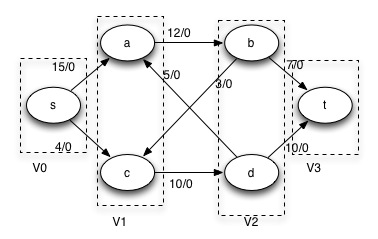
\includegraphics{diagrams/Chapter3_Example5_Solution.jpg} \\
\end{example}

\begin{theorem}
When the algorithm for layering stops in step 3, then the actual flow function has maximal total flow.
\end{theorem}

\begin{proof}
Determine a set S with $F = c(S)$. What S? \\
$ S = \bigcup_{i=0}^i V_j$, $\bar{S} = V \backslash S, s \in S, t \notin S$ \\ 
For any edge $ u \xrightarrow{e} v$, $e \in E_{S\bar{S}}$, we know $f(e) = c(e)$ because otherwise T would not be $\emptyset$. And for any edge $u \xleftarrow{e} v \in E_{\bar{S}S}$ we know $f(e) = 0$ and continue as for lemma 3.5.
\end{proof}